%
% Common preamble for all three parts.
%
\usepackage[T1]{fontenc}
\usepackage[utf8]{inputenc}
\usepackage[catalan]{babel}
\usepackage{amsmath}
\usepackage{color}
\usepackage{minted}
\usepackage{hyperref}
\usepackage{multicol}
\usepackage{tabularx, booktabs}
\usepackage{tikz}

% only inline todonotes work
\usepackage{xkeyval}
\usepackage[textsize=small]{todonotes}
\presetkeys{todonotes}{inline}{}

\usetikzlibrary{shapes,arrows,positioning,shadows}

% no nav buttons
\usenavigationsymbolstemplate{}

\newcommand{\bftt}[1]{\textbf{\texttt{#1}}}
\newcommand{\comment}[1]{{\color[HTML]{008080}\textit{\textbf{\texttt{#1}}}}}
\newcommand{\cmd}[1]{{\color[HTML]{008000}\bftt{#1}}}
\newcommand{\bs}{\char`\\}
\newcommand{\cmdbs}[1]{\cmd{\bs#1}}
\newcommand{\lcb}{\char '173}
\newcommand{\rcb}{\char '175}
\newcommand{\cmdbegin}[1]{\cmdbs{begin\lcb}\bftt{#1}\cmd{\rcb}}
\newcommand{\cmdend}[1]{\cmdbs{end\lcb}\bftt{#1}\cmd{\rcb}}

\newcommand{\wllogo}{\textbf{Overleaf}}

% this is where the example source files are loaded from
% do not include a trailing slash
\newcommand{\fileuri}{https://raw.github.com/pastells/curs-latex/master/ca}

\newcommand{\wlserver}{https://www.overleaf.com}
\newcommand{\wlnewdoc}[1]{\wlserver/docs?snip\_uri=\fileuri/#1\&splash=none}

\def\tikzname{Ti\emph{k}Z}

% from http://tex.stackexchange.com/questions/5226/keyboard-font-for-latex
\newcommand*\keystroke[1]{%
  \tikz[baseline=(key.base)]
    \node[%
      draw,
      fill=white,
      drop shadow={shadow xshift=0.25ex,shadow yshift=-0.25ex,fill=black,opacity=0.75},
      rectangle,
      rounded corners=2pt,
      inner sep=1pt,
      line width=0.5pt,
      font=\scriptsize\sffamily
    ](key) {#1\strut}
  ;
}
\newcommand{\keystrokebftt}[1]{\keystroke{\bftt{#1}}}

% stolen from minted.dtx
\newenvironment{exampletwoup}
  {\VerbatimEnvironment
   \begin{VerbatimOut}{example.out}}
  {\end{VerbatimOut}
   \setlength{\parindent}{0pt}
   \fbox{\begin{tabular}{l|l}
   \begin{minipage}{0.55\linewidth}
     \inputminted[fontsize=\small,resetmargins]{latex}{example.out}
   \end{minipage} &
   \begin{minipage}{0.35\linewidth}
     \input{example.out}
   \end{minipage}
   \end{tabular}}}

\newenvironment{exampletwouptiny}
  {\VerbatimEnvironment
   \begin{VerbatimOut}{example.out}}
  {\end{VerbatimOut}
   \setlength{\parindent}{0pt}
   \fbox{\begin{tabular}{l|l}
   \begin{minipage}{0.55\linewidth}
     \inputminted[fontsize=\scriptsize,resetmargins]{latex}{example.out}
   \end{minipage} &
   \begin{minipage}{0.35\linewidth}
     \setlength{\parskip}{6pt plus 1pt minus 1pt}%
     \raggedright\scriptsize\input{example.out}
   \end{minipage}
   \end{tabular}}}

\newenvironment{exampletwouptinynoframe}
  {\VerbatimEnvironment
   \begin{VerbatimOut}{example.out}}
  {\end{VerbatimOut}
   \setlength{\parindent}{0pt}
   \begin{tabular}{l|l}
   \begin{minipage}{0.55\linewidth}
     \inputminted[fontsize=\scriptsize,resetmargins]{latex}{example.out}
   \end{minipage} &
   \begin{minipage}{0.35\linewidth}
     \setlength{\parskip}{6pt plus 1pt minus 1pt}%
     \raggedright\scriptsize\input{example.out}
   \end{minipage}
   \end{tabular}}

\title{Introducció Interactiva a \LaTeX}
\author{Pol Pastells}
\titlegraphic{%

\includegraphics[height=24pt]{overleaf} \quad

\includegraphics[height=24pt]{logo_UB.png}
}

\date{17 de maig de 2024}

\subtitle{Tercera part}

\newcommand{\mar}[1]{\todo[color=green!40]{#1}}
\newcommand{\andreu}[1]{\todo[color=purple!40]{#1}}

\begin{document}

%%%%%%%%%%%%%%%%%%%%%%%%%%%%%%%%%%%%%%%%%%%%%%%%%%%%%%%%%%%%%%%%%%%%%%%%%%%%%%%
%%%%%%%%%%%%%%%%%%%%%%%%%%%%%%%%%%%%%%%%%%%%%%%%%%%%%%%%%%%%%%%%%%%%%%%%%%%%%%%
%%%%%%%%%%%%%%%%%%%%%%%%%%%%%%%%%%%%%%%%%%%%%%%%%%%%%%%%%%%%%%%%%%%%%%%%%%%%%%%
\begin{frame}
\titlepage{}
\end{frame}

%%%%%%%%%%%%%%%%%%%%%%%%%%%%%%%%%%%%%%%%%%%%%%%%%%%%%%%%%%%%%%%%%%%%%%%%%%%%%%%
%%%%%%%%%%%%%%%%%%%%%%%%%%%%%%%%%%%%%%%%%%%%%%%%%%%%%%%%%%%%%%%%%%%%%%%%%%%%%%%
%%%%%%%%%%%%%%%%%%%%%%%%%%%%%%%%%%%%%%%%%%%%%%%%%%%%%%%%%%%%%%%%%%%%%%%%%%%%%%%
\begin{frame}[fragile]{Repassem: Dubtes classe anterior}
\begin{itemize}
    \item \textbf{Com es referencia una secció pel seu nom?}\\
    El paquet \bftt{hyperref} també carrega l'ordre \cmdbs{nameref}.
\begin{exampletwouptiny}
\nameref{sec:exemples_ling}
\end{exampletwouptiny}
\end{itemize}
\end{frame}

%%%%%%%%%%%%%%%%%%%%%%%%%%%%%%%%%%%%%%%%%%%%%%%%%%%%%%%%%%%%%%%%%%%%%%%%%%%%%%%
%%%%%%%%%%%%%%%%%%%%%%%%%%%%%%%%%%%%%%%%%%%%%%%%%%%%%%%%%%%%%%%%%%%%%%%%%%%%%%%
%%%%%%%%%%%%%%%%%%%%%%%%%%%%%%%%%%%%%%%%%%%%%%%%%%%%%%%%%%%%%%%%%%%%%%%%%%%%%%%
\section{Anotacions amb \protect\bftt{todonotes}}
\begin{frame}{Continguts}
\begin{multicols}{2}
\tableofcontents[currentsection]
\end{multicols}
\end{frame}

%%%%%%%%%%%%%%%%%%%%%%%%%%%%%%%%%%%%%%%%%%%%%%%%%%%%%%%%%%%%%%%%%%%%%%%%%%%%%%%
%%%%%%%%%%%%%%%%%%%%%%%%%%%%%%%%%%%%%%%%%%%%%%%%%%%%%%%%%%%%%%%%%%%%%%%%%%%%%%%
%%%%%%%%%%%%%%%%%%%%%%%%%%%%%%%%%%%%%%%%%%%%%%%%%%%%%%%%%%%%%%%%%%%%%%%%%%%%%%%
\begin{frame}[fragile]{Anotacions amb \protect\bftt{todonotes}}
\begin{itemize}
\item L'ordre \cmdbs{todo} del paquet \bftt{todonotes} és útil per deixar notes
per a un mateix o per co"laboradors.
\begin{exampletwouptiny}
\todo{afegir resultats}
\todo[color=blue!20]{arreglar taula}
\end{exampletwouptiny}
\vskip 2ex
\item Fes-ho senzill: defineix les teves pròpies ordres amb \cmdbs{newcommand}
\begin{minted}[fontsize=\scriptsize,frame=single]{latex}
% el primer 1 marca que rep una variable (el text)
% #1 és la variable dins l'ordre
\newcommand{\mar}[1]{\todo[color=green!40]{#1}}
\newcommand{\andreu}[1]{\todo[color=purple!40]{#1}}
\end{minted}
Ja no cal escriure tant:
\begin{exampletwouptiny}
\mar{afegir resultats}
\andreu{arreglar taula}
\end{exampletwouptiny}
\end{itemize}
\end{frame}

%%%%%%%%%%%%%%%%%%%%%%%%%%%%%%%%%%%%%%%%%%%%%%%%%%%%%%%%%%%%%%%%%%%%%%%%%%%%%%%
%%%%%%%%%%%%%%%%%%%%%%%%%%%%%%%%%%%%%%%%%%%%%%%%%%%%%%%%%%%%%%%%%%%%%%%%%%%%%%%
%%%%%%%%%%%%%%%%%%%%%%%%%%%%%%%%%%%%%%%%%%%%%%%%%%%%%%%%%%%%%%%%%%%%%%%%%%%%%%%
\begin{frame}[fragile]{Anotacions amb \protect\bftt{todonotes}}
\begin{columns}
  \begin{column}{0.4\textwidth}
    \begin{itemize}
    \item Es poden enumerar les notes amb l'ordre \cmdbs{listoftodos}.
    \end{itemize}
  \end{column}
  \begin{column}{0.6\textwidth}
    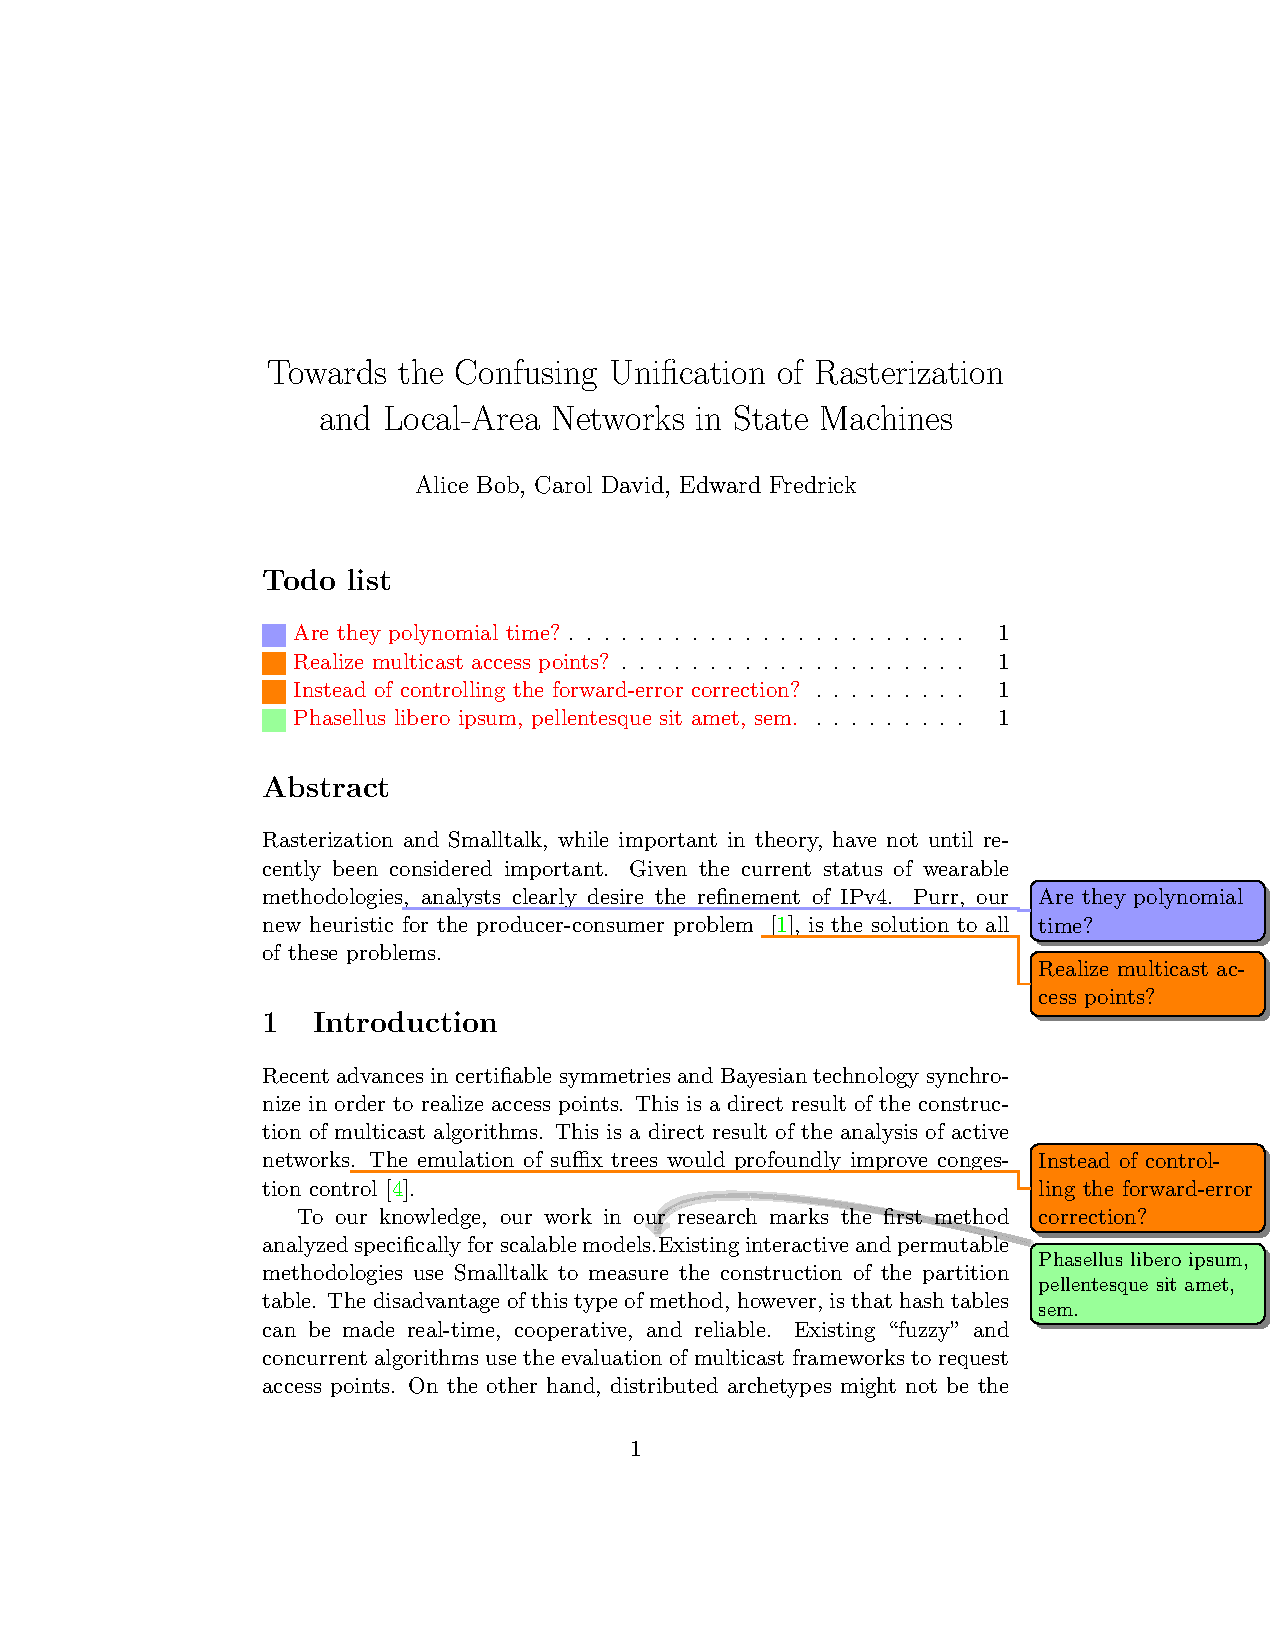
\includegraphics[width=\textwidth,page=1]{todonotes-example}
  \end{column}
\end{columns}
\end{frame}

%%%%%%%%%%%%%%%%%%%%%%%%%%%%%%%%%%%%%%%%%%%%%%%%%%%%%%%%%%%%%%%%%%%%%%%%%%%%%%%
%%%%%%%%%%%%%%%%%%%%%%%%%%%%%%%%%%%%%%%%%%%%%%%%%%%%%%%%%%%%%%%%%%%%%%%%%%%%%%%
%%%%%%%%%%%%%%%%%%%%%%%%%%%%%%%%%%%%%%%%%%%%%%%%%%%%%%%%%%%%%%%%%%%%%%%%%%%%%%%
\section{Transcripció fonètica}
\begin{frame}{Continguts}
\begin{multicols}{2}
\tableofcontents[currentsection]
\end{multicols}
\end{frame}

%%%%%%%%%%%%%%%%%%%%%%%%%%%%%%%%%%%%%%%%%%%%%%%%%%%%%%%%%%%%%%%%%%%%%%%%%%%%%%%
%%%%%%%%%%%%%%%%%%%%%%%%%%%%%%%%%%%%%%%%%%%%%%%%%%%%%%%%%%%%%%%%%%%%%%%%%%%%%%%
%%%%%%%%%%%%%%%%%%%%%%%%%%%%%%%%%%%%%%%%%%%%%%%%%%%%%%%%%%%%%%%%%%%%%%%%%%%%%%%
\begin{frame}[fragile]{tipa}
\begin{itemize}
    \item El paquet \bftt{tipa} facilita la introducció de símols de l'alfabet fonètic internacional. 
    \item Per símbols que no són un sol caràcter, es pot definir una nova variable al preàmbul. 
\end{itemize}

\begin{minipage}{0.45\linewidth}
\inputminted[fontsize=\tiny,frame=single,resetmargins]{latex}%
  {ipa.tex}
\end{minipage}
\hfill
\begin{minipage}{0.5\linewidth}

\includegraphics[width=\textwidth,clip,trim=1.5in 8in 4.5in 1.5in]{ipa.pdf}
\end{minipage}
\end{frame}

%%%%%%%%%%%%%%%%%%%%%%%%%%%%%%%%%%%%%%%%%%%%%%%%%%%%%%%%%%%%%%%%%%%
%%%%%%%%%%%%%%%%%%%%%%%%%%%%%%%%%%%%%%%%%%%%%%%%%%%%%%%%%%%%%%%%%%%%%%%%%%%%%%%
%%%%%%%%%%%%%%%%%%%%%%%%%%%%%%%%%%%%%%%%%%%%%%%%%%%%%%%%%%%%%%%%%%%%%%%%%%%%%%%
\begin{frame}[fragile]{tipauni}
\begin{itemize}
    \item És recomenable carregar el paquet \bftt{tipauni} en comptes de \bftt{tipa}. Funciona exactament igual, però ens permetrà copiar els caràcters en Unicode.
    \item Per defecte utilitza la font \emph{DoulosSIL}. Si voleu la mateixa font a tot el document, i que tingui negreta i cursiva, podeu fer servir \emph{charisSIL}.
    \item Vegeu \href{https://jon.dehdari.org/tutorials/tipachart_mod.pdf}{aquesta taula resum} per un resum dels símbols i diacrítics, o \href{https://ctan.org/pkg/tipa}{el manual de tipa} per la informació completa.
\end{itemize}
\end{frame}

%%%%%%%%%%%%%%%%%%%%%%%%%%%%%%%%%%%%%%%%%%%%%%%%%%%%%%%%%%%%%%%%%%%
%%%%%%%%%%%%%%%%%%%%%%%%%%%%%%%%%%%%%%%%%%%%%%%%%%%%%%%%%%%%%%%%%%%%%%%%%%%%%%%
%%%%%%%%%%%%%%%%%%%%%%%%%%%%%%%%%%%%%%%%%%%%%%%%%%%%%%%%%%%%%%%%%%%%%%%%%%%%%%%
\begin{frame}[fragile]{Incís: Fonts, Unicode, Xe\LaTeX{} i Lua\LaTeX{}}
\begin{itemize}
    \item És recomenable carregar el paquet \bftt{tipauni} en comptes de \bftt{tipa}. Funciona exactament igual, però ens permetrà copiar els caràcters en Unicode.
    \item Per defecte utilitza la font \emph{DoulosSIL}. Si voleu la mateixa font a tot el document, i que tingui negreta i cursiva, podeu fer servir \emph{charisSIL}.
\end{itemize}
\end{frame}

%%%%%%%%%%%%%%%%%%%%%%%%%%%%%%%%%%%%%%%%%%%%%%%%%%%%%%%%%%%%%%%%%%%%%%%%%%%%%%%
%%%%%%%%%%%%%%%%%%%%%%%%%%%%%%%%%%%%%%%%%%%%%%%%%%%%%%%%%%%%%%%%%%%%%%%%%%%%%%%
%%%%%%%%%%%%%%%%%%%%%%%%%%%%%%%%%%%%%%%%%%%%%%%%%%%%%%%%%%%%%%%%%%%%%%%%%%%%%%%
\begin{frame}[fragile]{Extra: diagrama vocals}
\begin{itemize}
\item El paquet \bftt{vowel} permet crear diagrames de vocals.
\end{itemize}
\begin{minipage}{0.55\linewidth}
\inputminted[fontsize=\tiny,frame=single,resetmargins]{latex}%
  {ipa-vowel.tex}
\end{minipage}
\hfill
\begin{minipage}{0.4\linewidth}

\includegraphics[width=\textwidth,clip,trim=2in 8.5in 4.5in 1.5in]{ipa-vowel.pdf}
\end{minipage}
\end{frame}

%%%%%%%%%%%%%%%%%%%%%%%%%%%%%%%%%%%%%%%%%%%%%%%%%%%%%%%%%%%%%%%%%%%%%%%%%%%%%%%
%%%%%%%%%%%%%%%%%%%%%%%%%%%%%%%%%%%%%%%%%%%%%%%%%%%%%%%%%%%%%%%%%%%%%%%%%%%%%%%
%%%%%%%%%%%%%%%%%%%%%%%%%%%%%%%%%%%%%%%%%%%%%%%%%%%%%%%%%%%%%%%%%%%%%%%%%%%%%%%
\section{Exemples lingüístics}\label{sec:exemples_ling}
\begin{frame}{Continguts}
\begin{multicols}{2}
\tableofcontents[currentsection]
\end{multicols}
\end{frame}


%%%%%%%%%%%%%%%%%%%%%%%%%%%%%%%%%%%%%%%%%%%%%%%%%%%%%%%%%%%%%%%%%%%%%%%%%%%%%%%
%%%%%%%%%%%%%%%%%%%%%%%%%%%%%%%%%%%%%%%%%%%%%%%%%%%%%%%%%%%%%%%%%%%%%%%%%%%%%%%
%%%%%%%%%%%%%%%%%%%%%%%%%%%%%%%%%%%%%%%%%%%%%%%%%%%%%%%%%%%%%%%%%%%%%%%%%%%%%%%
\begin{frame}[fragile]{linguex: exemples}
\begin{itemize}
\item Les 3 ordres bàsiques de linguex són \cmdbs{ex.}, \cmdbs{a.} i \cmdbs{b.}.
\item \cmdbs{ex.} inicia l'exemple, i \textbf{cal una línia en blanc} per acabar-lo.
\begin{exampletwouptiny2}
\ex. Exemple

\ex. Primer nivell de l'exemple
\a. Segon nivell de l'exemple
\b. Seguim al segon nivell

\ex.
\a. podem deixar buit
\b. el primer nivell
\c. si volem ser ordenats
\d. podem fer servir
\e. tot l'abecedari
\b. tot i que no cal

\end{exampletwouptiny2}
\item Les ordres \cmdbs{c.}, \cmdbs{d.}, etc.~són còpies de \cmdbs{b.}.
\item \bftt{linguex} és senzill, però, tot i poder-se modificar, és limitat. Hi ha paquets més potents però amb una sintaxi més complexa. \href{https://www.jostellings.com/numbex.html}{Vegeu aquesta breu explicació}.
\end{itemize}
\end{frame}

%%%%%%%%%%%%%%%%%%%%%%%%%%%%%%%%%%%%%%%%%%%%%%%%%%%%%%%%%%%%%%%%%%%%%%%%%%%%%%%
%%%%%%%%%%%%%%%%%%%%%%%%%%%%%%%%%%%%%%%%%%%%%%%%%%%%%%%%%%%%%%%%%%%%%%%%%%%%%%%
%%%%%%%%%%%%%%%%%%%%%%%%%%%%%%%%%%%%%%%%%%%%%%%%%%%%%%%%%%%%%%%%%%%%%%%%%%%%%%%
\begin{frame}[fragile]{linguex: referències}
\begin{itemize}
\item Podem fer servir \cmdbs{label} i \cmdbs{ref}.
\item També podem referir-nos als exemples més propers amb \cmdbs{Next}, \cmdbs{Last}, \cmdbs{NNext} i \cmdbs{LLast}, fins i tot si no tenen una etiqueta.
\end{itemize}
\begin{exampletwouptiny2}
A l'exemple~\ref{ex:1} hi ha faltes.
\ex. Ejenple
\label{ex:1}

\ex. Primer nivell de l'exemple
\a. Segon nivell de l'exemple

Com hem vist a \LLast i \Last \dots

En canvi a \Next i \NNext veiem \dots

\ex.
\a. podem deixar buit
\b. el primer nivell

\ex.
\label{ex:2}
\a. podem citar subexemples
\label{ex:2a}
\b. posant label a sota
\label{ex:2b}

Exemple \ref{ex:2} amb subexemples
\ref{ex:2a} i \ref{ex:2b}.

\end{exampletwouptiny2}
\end{frame}

%%%%%%%%%%%%%%%%%%%%%%%%%%%%%%%%%%%%%%%%%%%%%%%%%%%%%%%%%%%%%%%%%%%%%%%%%%%%%%%
%%%%%%%%%%%%%%%%%%%%%%%%%%%%%%%%%%%%%%%%%%%%%%%%%%%%%%%%%%%%%%%%%%%%%%%%%%%%%%%
%%%%%%%%%%%%%%%%%%%%%%%%%%%%%%%%%%%%%%%%%%%%%%%%%%%%%%%%%%%%%%%%%%%%%%%%%%%%%%%
\begin{frame}[fragile]{linguex: exemples 2}
\begin{itemize}
\item Per acabar un sol nivell s'utilitza \cmdbs{z.}
\begin{exampletwouptiny2}
\ex. Animals
\a. Gats
\a. miau
\z.
\b. Gossos
\a. bup
\z.
\b. Fures

\end{exampletwouptiny2}
\end{itemize}

\end{frame}

%%%%%%%%%%%%%%%%%%%%%%%%%%%%%%%%%%%%%%%%%%%%%%%%%%%%%%%%%%%%%%%%%%%%%%%%%%%%%%%
%%%%%%%%%%%%%%%%%%%%%%%%%%%%%%%%%%%%%%%%%%%%%%%%%%%%%%%%%%%%%%%%%%%%%%%%%%%%%%%
%%%%%%%%%%%%%%%%%%%%%%%%%%%%%%%%%%%%%%%%%%%%%%%%%%%%%%%%%%%%%%%%%%%%%%%%%%%%%%%
\begin{frame}[fragile]{linguex: gramaticalitat}
\begin{itemize}
    \item Linguex admet els símbols *, ?, \# i \% per judicis de gramaticalitat (els posa al davant)\footnote{recordeu que \# i \% s'escriuen amb una \keystroke{\textbackslash} davant}.
\begin{exampletwouptiny2}
\ex.
\a. Exemple ben format
\b. * Agramatical frase?
\b. ** i molt agramatical molt
\b. \# El formatge l'hi he posat
\c. ? Hi han maduixes

\end{exampletwouptiny2}
\end{itemize}

\end{frame}

%%%%%%%%%%%%%%%%%%%%%%%%%%%%%%%%%%%%%%%%%%%%%%%%%%%%%%%%%%%%%%%%%%%%%%%%%%%%%%%
%%%%%%%%%%%%%%%%%%%%%%%%%%%%%%%%%%%%%%%%%%%%%%%%%%%%%%%%%%%%%%%%%%%%%%%%%%%%%%%
%%%%%%%%%%%%%%%%%%%%%%%%%%%%%%%%%%%%%%%%%%%%%%%%%%%%%%%%%%%%%%%%%%%%%%%%%%%%%%%
\begin{frame}[fragile]{linguex: glosses}
\begin{itemize}
\item Linguex és molt últil per morfologia.
\item Per glossar un exemple afegim `g' després de l'última lletra de l'ordre i linguex s'encarrega d'alinear les paraules (cal \keystrokebftt{\bs\bs}  per marcar el final de línia).
\begin{exampletwouptiny2}
\ex.\a. No gloss
\bg. This is a first gloss\\
Dies ist eine erste Glosse\\

\exg.
Dies ist nicht die erste Glosse\\
This is not the first gloss\\

\end{exampletwouptiny2}
\item Podem afegir una tercera línia de traducció amb \cmdbs{glt} (gloss translation).
\begin{exampletwouptiny2}
\exg.
Martin-ek Diego-\zero{} ikusi du \\
Martin-ERG Diego-ABS vist ha \\
\glt `En Martin ha vist en Diego'

\end{exampletwouptiny2}
\end{itemize}

\end{frame}

%%%%%%%%%%%%%%%%%%%%%%%%%%%%%%%%%%%%%%%%%%%%%%%%%%%%%%%%%%%%%%%%%%%%%%%%%%%%%%%
%%%%%%%%%%%%%%%%%%%%%%%%%%%%%%%%%%%%%%%%%%%%%%%%%%%%%%%%%%%%%%%%%%%%%%%%%%%%%%%
%%%%%%%%%%%%%%%%%%%%%%%%%%%%%%%%%%%%%%%%%%%%%%%%%%%%%%%%%%%%%%%%%%%%%%%%%%%%%%%
\begin{frame}[fragile]{linguex: glosses 2}
\begin{itemize}
\item Podem modificar les glosses perquè tinguin l'aspecte que vulguem.
\begin{exampletwouptiny}
\renewcommand{\eachwordone}{\itshape}
\renewcommand{\eachwordtwo}{\tiny}

\exg.
Martin-ek Diego-\zero{} ikusi du \\
Martin-ERG Diego-ABS vist ha \\
\glt `En Martin ha vist en Diego'


\end{exampletwouptiny}
\end{itemize}

\end{frame}

%%%%%%%%%%%%%%%%%%%%%%%%%%%%%%%%%%%%%%%%%%%%%%%%%%%%%%%%%%%%%%%%%%%%%%%%%%%%%%%
%%%%%%%%%%%%%%%%%%%%%%%%%%%%%%%%%%%%%%%%%%%%%%%%%%%%%%%%%%%%%%%%%%%%%%%%%%%%%%%
%%%%%%%%%%%%%%%%%%%%%%%%%%%%%%%%%%%%%%%%%%%%%%%%%%%%%%%%%%%%%%%%%%%%%%%%%%%%%%%
\begin{frame}[fragile]{linguex: claudators}
\begin{itemize}
\item Amb l'ordre \cmdbs{exi.} es pot fer servir notació amb claudators
\item Si l'exemple conté una glossa, cal saltar-se elements amb `\{\}'
\begin{MyMinted}
\exi.
\a.  [SC that [ST John$_i$  [Sv $t_i$ likes Mary ]]]
\bg. [SC dass [ST Peter$_i$ [Sv $t_i$ Mari liebt ]]] \\
{} that {} Peter {} {} Mary loves \\
\glt `that Peter loves Mary'
\end{MyMinted}
\exi.
\a.  [SC that [ST John$_i$  [Sv $t_i$ likes Mary ]]]
\bg. [SC dass [ST Peter$_i$ [Sv $t_i$ Mari liebt ]]] \\
{} that {} Peter {} {} Mary loves \\
\glt `that Peter loves Mary'

\end{itemize}

\end{frame}

%%%%%%%%%%%%%%%%%%%%%%%%%%%%%%%%%%%%%%%%%%%%%%%%%%%%%%%%%%%%%%%%%%%%%%%%%%%%%%%
%%%%%%%%%%%%%%%%%%%%%%%%%%%%%%%%%%%%%%%%%%%%%%%%%%%%%%%%%%%%%%%%%%%%%%%%%%%%%%%
%%%%%%%%%%%%%%%%%%%%%%%%%%%%%%%%%%%%%%%%%%%%%%%%%%%%%%%%%%%%%%%%%%%%%%%%%%%%%%%
\begin{frame}[fragile]{Extra: arbres}
\begin{itemize}
\item Hi ha dos paquets importants per fer arbres: \bftt{forest} i \bftt{tikz-qtree}.
\item Mireu els manuals per saber quin uns convé.
\begin{exampletwouptiny}
\ex. \begin{forest}
[SC[C][ST[T][SV[V][SN]]]]
\end{forest}

\end{exampletwouptiny}
\item \href{https://ling.auf.net/lingbuzz/003391}{Guia forest}
\end{itemize}

\end{frame}




%%%%%%%%%%%%%%%%%%%%%%%%%%%%%%%%%%%%%%%%%%%%%%%%%%%%%%%%%%%%%%%%%%%%%%%%%%%%%%%
%%%%%%%%%%%%%%%%%%%%%%%%%%%%%%%%%%%%%%%%%%%%%%%%%%%%%%%%%%%%%%%%%%%%%%%%%%%%%%%
%%%%%%%%%%%%%%%%%%%%%%%%%%%%%%%%%%%%%%%%%%%%%%%%%%%%%%%%%%%%%%%%%%%%%%%%%%%%%%%
\section{Presentacions amb \protect\bftt{beamer}}

\begin{frame}{Continguts}
\begin{multicols}{2}
\tableofcontents[currentsection]
\end{multicols}
\end{frame}

%%%%%%%%%%%%%%%%%%%%%%%%%%%%%%%%%%%%%%%%%%%%%%%%%%%%%%%%%%%%%%%%%%%%%%%%%%%%%%%
%%%%%%%%%%%%%%%%%%%%%%%%%%%%%%%%%%%%%%%%%%%%%%%%%%%%%%%%%%%%%%%%%%%%%%%%%%%%%%%
%%%%%%%%%%%%%%%%%%%%%%%%%%%%%%%%%%%%%%%%%%%%%%%%%%%%%%%%%%%%%%%%%%%%%%%%%%%%%%%
\begin{frame}[fragile]{Presentacions amb \protect\bftt{beamer}}
\begin{itemize}
\item Beamer és un paquet per fer presentacions (com aquesta).
\item Es fa servir amb el tipus de document \bftt{beamer}. Carrega automàticament alguns paquets, com \bftt{graphicx}, \bftt{hyperref} i \bftt{xcolor}.
\item L'entorn \bftt{frame} crea diapositives.
\end{itemize}
\begin{minipage}{0.55\linewidth}
\inputminted[fontsize=\scriptsize,frame=single,resetmargins]{latex}%
  {beamer-minimal.tex}
\end{minipage}
\begin{minipage}{0.35\linewidth}
% trim: l b r t
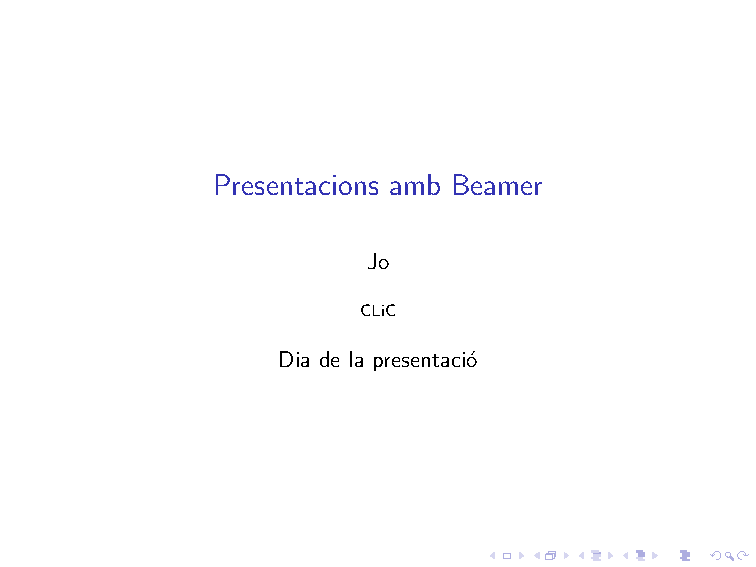
\includegraphics[width=\textwidth,clip,trim=1in 1in 1in 1in]{beamer-minimal.pdf}
\end{minipage}
\end{frame}

%%%%%%%%%%%%%%%%%%%%%%%%%%%%%%%%%%%%%%%%%%%%%%%%%%%%%%%%%%%%%%%%%%%%%%%%%%%%%%%
%%%%%%%%%%%%%%%%%%%%%%%%%%%%%%%%%%%%%%%%%%%%%%%%%%%%%%%%%%%%%%%%%%%%%%%%%%%%%%%
%%%%%%%%%%%%%%%%%%%%%%%%%%%%%%%%%%%%%%%%%%%%%%%%%%%%%%%%%%%%%%%%%%%%%%%%%%%%%%%
\begin{frame}[fragile]{Presentacions amb \protect\bftt{beamer}}

\begin{itemize}
\item Podeu partir de l'exemple i anar provant coses.
\end{itemize}
\vskip 2ex
\begin{center}
\fbox{\href{\wlnewdoc{beamer-minimal.tex}}{%
Cliqueu per obrir el document d'exemple a \wllogo{}}}
\end{center}
\end{frame}

%%%%%%%%%%%%%%%%%%%%%%%%%%%%%%%%%%%%%%%%%%%%%%%%%%%%%%%%%%%%%%%%%%%%%%%%%%%%%%%
%%%%%%%%%%%%%%%%%%%%%%%%%%%%%%%%%%%%%%%%%%%%%%%%%%%%%%%%%%%%%%%%%%%%%%%%%%%%%%%
%%%%%%%%%%%%%%%%%%%%%%%%%%%%%%%%%%%%%%%%%%%%%%%%%%%%%%%%%%%%%%%%%%%%%%%%%%%%%%%
\begin{frame}[fragile]
\frametitle{Presentacions amb \protect\bftt{beamer}: Marcs}
\begin{itemize}
\item \cmdbs{frametitle} posa el títol de la diapositiva.
\item Afegeix més continguts 
\item El codi per aquest requadres és: 
\vskip 2ex
\inputminted[fontsize=\scriptsize,frame=single,resetmargins]{latex}%
  {beamer-frame.tex}
\end{itemize}
\end{frame}

%%%%%%%%%%%%%%%%%%%%%%%%%%%%%%%%%%%%%%%%%%%%%%%%%%%%%%%%%%%%%%%%%%%%%%%%%%%%%%%
%%%%%%%%%%%%%%%%%%%%%%%%%%%%%%%%%%%%%%%%%%%%%%%%%%%%%%%%%%%%%%%%%%%%%%%%%%%%%%%
%%%%%%%%%%%%%%%%%%%%%%%%%%%%%%%%%%%%%%%%%%%%%%%%%%%%%%%%%%%%%%%%%%%%%%%%%%%%%%%
\begin{frame}[fragile]{Presentacions amb \protect\bftt{beamer}: Seccions}
\begin{itemize}
    \item Es poden agrupar els \bftt{frame}s en \cmdbs{section}s. \bftt{beamer} les farà servir per crear l'índex. 
    \item L'índex es crea amb \cmdbs{tableofcontents} igual que per articles.
    \item L'opció \bftt{currentsection} destaca la secció actual. 
\vskip 2ex
\begin{exampletwouptiny}
% comentaris

% per

% guanyar

% espai

% a la dreta

\tableofcontents[currentsection]
\end{exampletwouptiny}
\end{itemize}
\end{frame}

%%%%%%%%%%%%%%%%%%%%%%%%%%%%%%%%%%%%%%%%%%%%%%%%%%%%%%%%%%%%%%%%%%%%%%%%%%%%%%%
%%%%%%%%%%%%%%%%%%%%%%%%%%%%%%%%%%%%%%%%%%%%%%%%%%%%%%%%%%%%%%%%%%%%%%%%%%%%%%%
%%%%%%%%%%%%%%%%%%%%%%%%%%%%%%%%%%%%%%%%%%%%%%%%%%%%%%%%%%%%%%%%%%%%%%%%%%%%%%%
\begin{frame}[fragile]{Presentacions amb \protect\bftt{beamer}: Columnes}
Hi ha diverses maneres de dividir una diapositiva en columnes.
\begin{columns}
\begin{column}{0.4\textwidth}
\begin{enumerate}
\item Els entorns \bftt{columns} i \bftt{column} en són una.
      L'argument per cada \bftt{column} determina la seva amplada. 
\item El paquet \bftt{multicol} automàticament divideix un text en columnes. 
\end{enumerate}
\end{column}
\begin{column}{0.6\textwidth}
\begin{minted}[fontsize=\scriptsize,frame=single]{latex}
\begin{columns}
  \begin{column}{0.4\textwidth}
    \begin{itemize}
    \item Contingut de la  
    \item columna de  
    \item l'esquerra 
    \end{itemize}
  \end{column}
  \begin{column}{0.6\textwidth}
    % segona columna 
  \end{column}
\end{columns}
\end{minted}
\end{column}
\end{columns}
\end{frame}

%%%%%%%%%%%%%%%%%%%%%%%%%%%%%%%%%%%%%%%%%%%%%%%%%%%%%%%%%%%%%%%%%%%%%%%%%%%%%%%
%%%%%%%%%%%%%%%%%%%%%%%%%%%%%%%%%%%%%%%%%%%%%%%%%%%%%%%%%%%%%%%%%%%%%%%%%%%%%%%
%%%%%%%%%%%%%%%%%%%%%%%%%%%%%%%%%%%%%%%%%%%%%%%%%%%%%%%%%%%%%%%%%%%%%%%%%%%%%%%
\begin{frame}[fragile]{Presentacions amb \protect\bftt{beamer}: Destacar}
\begin{itemize}

\item \cmdbs{emph} o \cmdbs{alert} per destacar.
\vskip 1ex
\begin{exampletwouptiny}
Vull \emph{emfatitzar} que
soc un text \alert{important}.
\end{exampletwouptiny}
\vskip 1ex

\item Òbviament segueixen existint les ordres que ja hem vist per articles: 
\vskip 1ex
\begin{exampletwouptiny}
Text en \textbf{negreta}.
Text en \textit{cursiva}.
\end{exampletwouptiny}
\vskip 1ex

\item I podem fer servir colors\footnote{\bftt{beamer} carrega automàticament \href{https://ctan.javinator9889.com/macros/latex/contrib/xcolor/xcolor.pdf}{xcolor}, que té una àmplia paleta de colors, o ens podem definir els nostres propis. Per passar una opció a \bftt{xcolor} la podem passar directament a \bftt{beamer}, com \textbackslash documentclass[x11names]\{beamer\}.}
\vskip 1ex
\begin{exampletwouptiny}
Algo \textcolor{RoyalBlue1}{a destacar}
o \textcolor{DarkSeaGreen4}{diferent}.
\end{exampletwouptiny}
\vskip 1ex
\end{itemize}
\end{frame}

%%%%%%%%%%%%%%%%%%%%%%%%%%%%%%%%%%%%%%%%%%%%%%%%%%%%%%%%%%%%%%%%%%%%%%%%%%%%%%%
%%%%%%%%%%%%%%%%%%%%%%%%%%%%%%%%%%%%%%%%%%%%%%%%%%%%%%%%%%%%%%%%%%%%%%%%%%%%%%%
%%%%%%%%%%%%%%%%%%%%%%%%%%%%%%%%%%%%%%%%%%%%%%%%%%%%%%%%%%%%%%%%%%%%%%%%%%%%%%%
\begin{frame}[fragile]{Presentacions amb \protect\bftt{beamer}: Imatges}
\begin{itemize}
\item \cmdbs{includegraphics} del paquet \bftt{graphicx}.
\item L'entorn \bftt{figure} centra la imatge per defecta a \bftt{beamer}.
\vskip 2ex
\begin{exampletwouptiny}
\begin{figure}

\includegraphics[
  width=0.5\textwidth]{gus_gran}
  \caption{En Gus}
  \label{fig:gus}
\end{figure}
\end{exampletwouptiny}
\end{itemize}

\end{frame}

%%%%%%%%%%%%%%%%%%%%%%%%%%%%%%%%%%%%%%%%%%%%%%%%%%%%%%%%%%%%%%%%%%%%%%%%%%%%%%%
%%%%%%%%%%%%%%%%%%%%%%%%%%%%%%%%%%%%%%%%%%%%%%%%%%%%%%%%%%%%%%%%%%%%%%%%%%%%%%%
%%%%%%%%%%%%%%%%%%%%%%%%%%%%%%%%%%%%%%%%%%%%%%%%%%%%%%%%%%%%%%%%%%%%%%%%%%%%%%%
\begin{frame}[fragile]{Presentacions amb \protect\bftt{beamer}: Blocks}
\begin{itemize}
\item L'entorn \bftt{block} fa capses amb títol. 
\begin{exampletwouptiny}
\begin{block}{Dades interessants}
Resultats importants.
\end{block}

\begin{alertblock}{Compte}
    Pot ser important.
\end{alertblock}
\end{exampletwouptiny}

\item De la mateixa manera que \cmdbs{emph}, l'aspecte dels blocks dependrà del tema de \bftt{beamer}.
\end{itemize}
\end{frame}

%%%%%%%%%%%%%%%%%%%%%%%%%%%%%%%%%%%%%%%%%%%%%%%%%%%%%%%%%%%%%%%%%%%%%%%%%%%%%%%
%%%%%%%%%%%%%%%%%%%%%%%%%%%%%%%%%%%%%%%%%%%%%%%%%%%%%%%%%%%%%%%%%%%%%%%%%%%%%%%
%%%%%%%%%%%%%%%%%%%%%%%%%%%%%%%%%%%%%%%%%%%%%%%%%%%%%%%%%%%%%%%%%%%%%%%%%%%%%%%
\begin{frame}[fragile]
    \frametitle{Presentacions amb \protect\bftt{beamer}: Temes}
\begin{itemize}
    \item Es pot canviar el tema (aspecte). La majoria de temes clàssics de \LaTeX{} són tirant a lletjos, però s'en poden trobar de \href{https://github.com/martinbjeldbak/ultimate-beamer-theme-list?tab=readme-ov-file}{moderns} més decents. Aquesta presentació fa servir el tema \textbf{metropolis}.\footnote{Segons quin tema trobeu en línia, és possible que no estigui instalat a Overleaf o la vostra instalació local. En aquest cas caldrà descarrear-se'l i posar-lo a la mateixa carpeta del projecte.}
    \item O podeu veure exemples a \href{https://www.overleaf.com/gallery/tagged/beamer}{Overleaf}.
\end{itemize}
\begin{minipage}{0.55\linewidth}
\inputminted[fontsize=\scriptsize,frame=single,resetmargins]{latex}%
  {beamer-theme.tex}
\end{minipage}
\begin{minipage}{0.35\linewidth}
% trim: l b r t
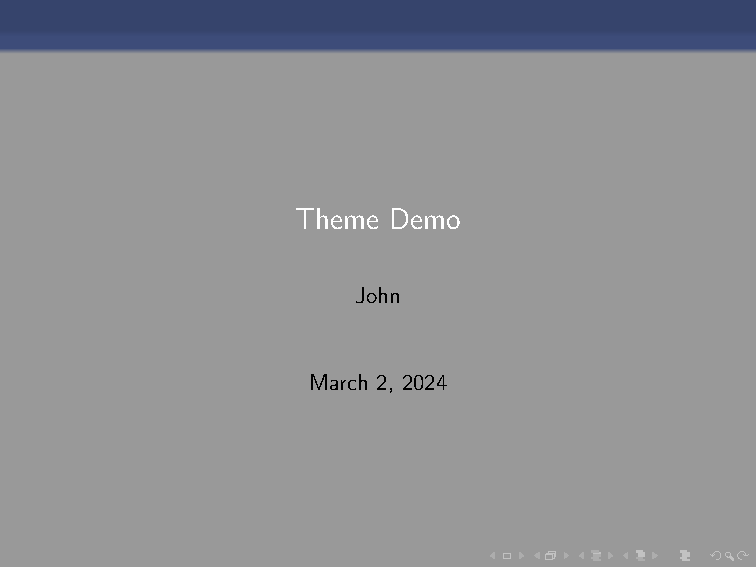
\includegraphics[width=\textwidth]{beamer-theme.pdf}
\end{minipage}
\end{frame}

%%%%%%%%%%%%%%%%%%%%%%%%%%%%%%%%%%%%%%%%%%%%%%%%%%%%%%%%%%%%%%%%%%%%%%%%%%%%%%%
%%%%%%%%%%%%%%%%%%%%%%%%%%%%%%%%%%%%%%%%%%%%%%%%%%%%%%%%%%%%%%%%%%%%%%%%%%%%%%%
%%%%%%%%%%%%%%%%%%%%%%%%%%%%%%%%%%%%%%%%%%%%%%%%%%%%%%%%%%%%%%%%%%%%%%%%%%%%%%%
\begin{frame}[fragile]{Presentacions amb \protect\bftt{beamer}: Animacions}
\begin{itemize}
    \item Un \bftt{frame} pot generar diverses diapositives.
    \item L'ordre \cmdbs{pause} mostra talla la diapositiva al punt on apareix. 
\vskip 2ex
\begin{exampletwouptinynoframe}
\begin{itemize}
\item Pots sentir la
\pause \item intriga?
\end{itemize}
\end{exampletwouptinynoframe}
\vskip 2ex
\item Hi ha més maneres de fer animacions a \bftt{beamer}; vegeu
les ordres \cmdbs{only}, \cmdbs{alt}, i \cmdbs{uncover}.
\end{itemize}
\end{frame}

%%%%%%%%%%%%%%%%%%%%%%%%%%%%%%%%%%%%%%%%%%%%%%%%%%%%%%%%%%%%%%%%%%%%%%%%%%%%%%%
%%%%%%%%%%%%%%%%%%%%%%%%%%%%%%%%%%%%%%%%%%%%%%%%%%%%%%%%%%%%%%%%%%%%%%%%%%%%%%%
%%%%%%%%%%%%%%%%%%%%%%%%%%%%%%%%%%%%%%%%%%%%%%%%%%%%%%%%%%%%%%%%%%%%%%%%%%%%%%%
\begin{frame}[fragile]{Presentacions amb \protect\bftt{beamer}: Exercici}

Recreeu la ``Gettysburg Powerpoint Presentation'' amb \bftt{beamer}.\footnote{\url{http://norvig.com/Gettysburg}}

\begin{enumerate}
\item Obriu l'exercici:
\begin{center}
\fbox{\href{\wlnewdoc{beamer-exercise.tex}}{%
Cliqueu per obrir l'exercici a \wllogo{}}}
\end{center}
\vskip 2ex
\item Descarregueu-vos la imatge \wllogo{} via the
files menu.
\begin{center}
\fbox{\href{\fileuri/figures/gettysburg_graph.png?dl=1}{Cliqueu per descarregar la imatge}}
\end{center}
\vskip 2ex
\item Feu que el document s'assembli al següent:
\begin{center}
\fbox{\href{\fileuri/beamer-exercise-solution.pdf}{%
Cliqueu per obrir el document model}}
\vfill
\fbox{\href{\wlnewdoc{beamer-exercise-solution.tex}}{%
Podeu veure la solució aquí}}
\end{center}
\end{enumerate}
\end{frame}

%%%%%%%%%%%%%%%%%%%%%%%%%%%%%%%%%%%%%%%%%%%%%%%%%%%%%%%%%%%%%%%%%%%%%%%%%%%%%%%
%%%%%%%%%%%%%%%%%%%%%%%%%%%%%%%%%%%%%%%%%%%%%%%%%%%%%%%%%%%%%%%%%%%%%%%%%%%%%%%
%%%%%%%%%%%%%%%%%%%%%%%%%%%%%%%%%%%%%%%%%%%%%%%%%%%%%%%%%%%%%%%%%%%%%%%%%%%%%%%
\section{Què més?}\label{sec:altres}
\begin{frame}{Continguts}
\begin{multicols}{2}
\tableofcontents[currentsection]
\end{multicols}
\end{frame}

%%%%%%%%%%%%%%%%%%%%%%%%%%%%%%%%%%%%%%%%%%%%%%%%%%%%%%%%%%%%%%%%%%%%%%%%%%%%%%%
%%%%%%%%%%%%%%%%%%%%%%%%%%%%%%%%%%%%%%%%%%%%%%%%%%%%%%%%%%%%%%%%%%%%%%%%%%%%%%%
%%%%%%%%%%%%%%%%%%%%%%%%%%%%%%%%%%%%%%%%%%%%%%%%%%%%%%%%%%%%%%%%%%%%%%%%%%%%%%%
\subsection{Altres coses interessants}
\begin{frame}[fragile]{Altres}
\begin{itemize}\small
    \item \cmdbs{\textbackslash} força canvi de línia i \cmdbs{newpage} canvi de pàgina (\href{https://www.overleaf.com/learn/latex/Line_breaks_and_blank_spaces#Line_breaks}{més sobre espaiat}).
    \item La titlla (``virguililla, tilde'') \keystroke{\~} és un caràcter especial a \LaTeX{}, cal escapar-la si es vol impresa. Es fa servir per evitar separar dues paraules en línies diferents (non-breaking space). És recomenable fer-la servir entre el nom i la referència.
    \item Típicament, una frase acaba en lletra minúscula seguida de punt. \LaTeX{} interpreta lletra majúscula seguida de punt com a acrònim. Si això no es compleix cal explicitar-ho per tenir l'espaiat adequat\footnote{La secció de bibliografia ja té això en compte.}:
    \begin{itemize}
        \item \cmd{.\textbackslash} marca un punt que no acaba la frase.
        \item \cmdbs{@} marca que una majúscula acaba la frase.
    \end{itemize}

\begin{exampletwouptiny}
Figura~\ref{fig:gus} \\
entre 0 i~1 \\
Donald~E. Knuth \\
Prof.~Adam\\
Treballa a l'ONU\@ \\
El ``Combin.\ Journal''
\end{exampletwouptiny}
\end{itemize}
\end{frame}

%%%%%%%%%%%%%%%%%%%%%%%%%%%%%%%%%%%%%%%%%%%%%%%%%%%%%%%%%%%%%%%%%%%%%%%%%%%%%%%
%%%%%%%%%%%%%%%%%%%%%%%%%%%%%%%%%%%%%%%%%%%%%%%%%%%%%%%%%%%%%%%%%%%%%%%%%%%%%%%
%%%%%%%%%%%%%%%%%%%%%%%%%%%%%%%%%%%%%%%%%%%%%%%%%%%%%%%%%%%%%%%%%%%%%%%%%%%%%%%
\begin{frame}[fragile]{Altres 2}
\begin{itemize}
    \item \cmdbs{footnote} per notes al peu de pàgina.
    \item \cmdbs{input} permet incloure documents de \LaTeX{} dins d'altres documents.
    Útil per:
        \begin{itemize}{\footnotesize
        \item Seccions de documents
        \item Taules complexes
        \item Separar el preàmbul (i reutilitzar-lo)
        }\end{itemize}
        \footnotesize{Vegeu \textit{treball morfologia basca} als exemples finals.}
        També hi ha
        \href{https://www.overleaf.com/learn/latex/Management_in_a_large_project}{altres opcions per tractar amb documents grans}.
    \item \normalsize Podem canviar la indentació dels paràgrafs (\href{https://www.overleaf.com/learn/latex/Articles/How_to_change_paragraph_spacing_in_LaTeX}{més sobre espaiat de paràgrafs}). \\
    \footnotesize{Vegeu \textit{treball de transcripció fonètica} als exemples finals.}
\begin{exampletiny}
%  Treu el sagnat
\setlength{\parindent}{0pt}
%  Passada la \tableofcontents afegeix espai en blanc
\setlength{\parskip}{\baselineskip}
\end{exampletiny}
\end{itemize}
\end{frame}
%%%%%%%%%%%%%%%%%%%%%%%%%%%%%%%%%%%%%%%%%%%%%%%%%%%%%%%%%%%%%%%%%%%%%%%%%%%%%%%
%%%%%%%%%%%%%%%%%%%%%%%%%%%%%%%%%%%%%%%%%%%%%%%%%%%%%%%%%%%%%%%%%%%%%%%%%%%%%%%
%%%%%%%%%%%%%%%%%%%%%%%%%%%%%%%%%%%%%%%%%%%%%%%%%%%%%%%%%%%%%%%%%%%%%%%%%%%%%%%
\subsection{Altres paquets}
\begin{frame}{Altres paquets i recursos}
\begin{itemize}
    \item \bftt{tikz}: per crear gràfics, una mica difícil.
    \item \bftt{langnames}: per noms d'idiomes de manera sistemàtica.
    \item \url{https://meluhha.com/tableau/} per taules de ``optimality theory''
    \item \href{https://detexify.kirelabs.org/classify.html}{Detexify} --- dibuixes el símbol i et diu com fer-lo amb \LaTeX.
    \item \href{https://tug.ctan.org/info/symbols/comprehensive/symbols-a4.pdf}{Llista de símbols que es poden fer a \LaTeX}.
    \item \href{https://arxiv.org}{arxiv} permet descarregar-se l'article amb \LaTeX de la majoria d'articles.
\end{itemize}
Vegeu \url{https://www.overleaf.com/latex/examples} i \url{http://texample.net} 
per exemples.
\end{frame}

%%%%%%%%%%%%%%%%%%%%%%%%%%%%%%%%%%%%%%%%%%%%%%%%%%%%%%%%%%%%%%%%%%%%%%%%%%%%%%%
%%%%%%%%%%%%%%%%%%%%%%%%%%%%%%%%%%%%%%%%%%%%%%%%%%%%%%%%%%%%%%%%%%%%%%%%%%%%%%%
%%%%%%%%%%%%%%%%%%%%%%%%%%%%%%%%%%%%%%%%%%%%%%%%%%%%%%%%%%%%%%%%%%%%%%%%%%%%%%%
\subsection{Instalar \LaTeX{}}
\begin{frame}{Instalar \LaTeX}
\begin{itemize}
\item Per fer servir \LaTeX{} al vostre ordinador, us caldrà una \emph{distribució}:
    inclou el programa \bftt{latex} i un munt de paquets.
\begin{itemize}
\item Windows: \href{http://miktex.org/}{Mik\TeX} o \href{http://tug.org/texlive/}{\TeX Live}
\item Linux: \href{http://tug.org/texlive/}{\TeX Live}
\item Mac: \href{http://tug.org/mactex/}{Mac\TeX}
\end{itemize}
\item També us caldrà un editor amb suport per \LaTeX{}. A \url{http://en.wikipedia.org/wiki/Comparison_of_TeX_editors} hi teniu una llista exhaustiva.
\end{itemize}
\end{frame}

%%%%%%%%%%%%%%%%%%%%%%%%%%%%%%%%%%%%%%%%%%%%%%%%%%%%%%%%%%%%%%%%%%%%%%%%%%%%%%%
%%%%%%%%%%%%%%%%%%%%%%%%%%%%%%%%%%%%%%%%%%%%%%%%%%%%%%%%%%%%%%%%%%%%%%%%%%%%%%%
%%%%%%%%%%%%%%%%%%%%%%%%%%%%%%%%%%%%%%%%%%%%%%%%%%%%%%%%%%%%%%%%%%%%%%%%%%%%%%%
\subsection{Exemples comentats}\label{sec:exemples_comentats}
\begin{frame}{Exemples comentats}
De senzill a complex:
\begin{itemize}
    \item \href{https://www.overleaf.com/read/rgxbsfvqsgbw\#ba04b9}{Breu transcripció fonètica} --- amb \bftt{tipauni} o \bftt{tipa} (comentat).
    \item \href{https://www.overleaf.com/read/mxysfjcnnppm\#294a25}{Treball de transcripció fonètica} --- més extens que l'anterior, barreja de \bftt{tipa} i unicode.
    \item \href{https://www.overleaf.com/read/sxkcdfrpmbcb\#10abd3}{Treball morfologia basca} --- conté:
\begin{itemize}
    \item Un treball estructurat amb diversos fitxers, glosses personalitzades, taules amb format avançat i exemples de bibliografia tant amb biblatex com amb apacite.
    \item Una presentació amb \bftt{beamer}.
\end{itemize}
\end{itemize}

Finalment, us pot ser útil \href{https://www.overleaf.com/read/zkfhtdnpbdwq\#2f636f}{aquesta plantilla senzilla}.

\end{frame}

%%%%%%%%%%%%%%%%%%%%%%%%%%%%%%%%%%%%%%%%%%%%%%%%%%%%%%%%%%%%%%%%%%%%%%%%%%%%%%%
%%%%%%%%%%%%%%%%%%%%%%%%%%%%%%%%%%%%%%%%%%%%%%%%%%%%%%%%%%%%%%%%%%%%%%%%%%%%%%%
%%%%%%%%%%%%%%%%%%%%%%%%%%%%%%%%%%%%%%%%%%%%%%%%%%%%%%%%%%%%%%%%%%%%%%%%%%%%%%%
\subsection{Referències en línia}
\begin{frame}{Referències en línia}
\begin{itemize}
\item \href{https://www.overleaf.com/learn}{The Overleaf Learn Wiki} --- tutorials i material de referència.
\item \href{http://en.wikibooks.org/wiki/LaTeX}{The \LaTeX{} Wikibook} --- més tutorials i material de referència.
\item \href{http://tex.stackexchange.com/}{\TeX{} Stack Exchange} --- preguntes i respostes
\item \href{http://www.latex-community.org/}{\LaTeX{} Community} --- fòrum
\item \href{http://ctan.org/}{Comprehensive \TeX{} Archive Network (CTAN)} --- documentació de paquets.
\item Qualsevol buscador us portarà a alguna d'aquestes pàgines.
\end{itemize}

Repositori del curs: \href{https://github.com/Pastells/curs-latex}{Pastells/curs-latex}
\end{frame}


%%%%%%%%%%%%%%%%%%%%%%%%%%%%%%%%%%%%%%%%%%%%%%%%%%%%%%%%%%%%%%%%%%%%%%%%%%%%%%%
%%%%%%%%%%%%%%%%%%%%%%%%%%%%%%%%%%%%%%%%%%%%%%%%%%%%%%%%%%%%%%%%%%%%%%%%%%%%%%%
%%%%%%%%%%%%%%%%%%%%%%%%%%%%%%%%%%%%%%%%%%%%%%%%%%%%%%%%%%%%%%%%%%%%%%%%%%%%%%%
\begin{frame}[standout]
\Huge Gràcies!
\end{frame}

\end{document}
